\documentclass[12pt, twoside]{article}
\documentclass[12pt, twoside]{article}
\usepackage[letterpaper, margin=1in, headsep=0.2in]{geometry}
\setlength{\headheight}{0.6in}
%\usepackage[english]{babel}
\usepackage[utf8]{inputenc}
\usepackage{microtype}
\usepackage{amsmath}
\usepackage{amssymb}
%\usepackage{amsfonts}
\usepackage{siunitx} %units in math. eg 20\milli\meter
\usepackage{yhmath} % for arcs, overparenth command
\usepackage{tikz} %graphics
\usetikzlibrary{quotes, angles}
\usepackage{graphicx} %consider setting \graphicspath{{images/}}
\usepackage{parskip} %no paragraph indent
\usepackage{enumitem}
\usepackage{multicol}
\usepackage{venndiagram}

\usepackage{fancyhdr}
\pagestyle{fancy}
\fancyhf{}
\renewcommand{\headrulewidth}{0pt} % disable the underline of the header
\raggedbottom
\hfuzz=2mm %suppresses overfull box warnings

\usepackage{hyperref}

\title{PreCalculus}
\author{Chris Huson}
\date{March 2023}

\fancyhead[LE]{\thepage}
\fancyhead[RO]{\thepage \\ Name: \hspace{3cm} \,\\}
\fancyhead[LO]{BECA / Huson / Unit 11: Calculus \\* 26 April 2023}

\begin{document}

\subsubsection*{11.9 Pre-Quiz: Tangent and normal lines to a function}
Use your own notebook, but no calculators or computers

\begin{enumerate}

\subsubsection*{Find the derivative of each polynomial function}
\item $f(x)=x^2+5x$ \vspace{3cm}
\item $f(x)=x^4-2x^3+7x^2-11$ \par \vspace{3cm}

\textbf{Evaluate the function and its derivative at a given point}
\item Given $f(x)=2x^2-x+3$
\begin{enumerate}[itemsep=3cm]
    \item Find $f(2)$
    \item Find $f'(2)$
\end{enumerate} \vspace{2cm}

\newpage
\item The graph shows the polynomial function $\displaystyle y=x^3-x^2-3x+2$. Its derivative is $\displaystyle \frac{dy}{dx}=3x^2-2x-3$. 
\begin{multicols}{2}
    \begin{enumerate}[itemsep=1cm]
        \item Write down the coordinates of the point $P$.
        \item Find the slope of the tangent line at $P$.
        \item Write down the equation of the tangent line at $P$.
        \item Draw the tangent line on the graph accurately with a straight edge.
    \end{enumerate}
        \begin{center}
    \begin{tikzpicture}[x=1cm, y=1cm, scale=1]
        \draw [thin, color=lightgray, xstep=1.0cm,ystep=1.0cm] (-3,-3.1) grid (4,5);
        \draw [thick, ->] (-3,0) -- (+4.3,0) node [above left]{$x$};
        \draw [thick, ->] (0,-3.2) -- (0,5.2) node [right]{$y$};
        \foreach \x in {-3,...,4}
            \draw (\x cm,0) -- (\x cm,0) node[below] {$\x$};
        \foreach \y in {-3,-2,...,5}
            \draw[shift={(0,\y)}] (2pt,0pt)--(-2pt,0pt) node[left]{$\y$};
        \draw [thick,<->,smooth,domain=-1.8:2.5] plot(\x,{(\x*\x*\x-\x*\x-3*\x+2)});
        \fill (1,-1) circle[radius=0.1] node[below left]{$P$};
    \end{tikzpicture}
    \end{center}
\end{multicols}

\item The function $y=-x^2+3x+2$ is graphed on the grid below. Find its derivative and the equations of the tangent and normal lines through point $(1,5)$. Draw the lines.
    \begin{flushright}
        \begin{tikzpicture}[x=1cm, y=1cm, scale=0.9]
            \draw [thin, color=lightgray, xstep=1.0cm,ystep=1.0cm] (-2,-2) grid (5,8);
            \draw [thick, ->] (-2,0) -- (+5.3,0) node [above right]{$x$};
            \draw [thick, ->] (0,-2) -- (0,8.3) node [right]{$y$};
            \foreach \x in {-2,...,5}
                \draw (\x cm,0) -- (\x cm,0) node[below] {$\x$};
            \foreach \y in {-2,...,8}
                \draw[shift={(0,\y)}] (2pt,0pt)--(-2pt,0pt) node[left]{$\y$};
            \draw [thick,<->,smooth,domain=-1.3:4.3] plot(\x,{(-\x*\x+3*\x+3)});
        \end{tikzpicture}
    \end{flushright}


\end{enumerate}
\end{document}



